%%%%%%%%%%%%%%%%%%%%% chapter.tex %%%%%%%%%%%%%%%%%%%%%%%%%%%%%%%%%
%
% sample chapter
%
% Use this file as a template for your own input.
%
%%%%%%%%%%%%%%%%%%%%%%%% Springer-Verlag %%%%%%%%%%%%%%%%%%%%%%%%%%
%\motto{Use the template \emph{chapter.tex} to style the various elements of your chapter content.}
\chapter{Residue Calculus}
\label{ResCalc} % Always give a unique label
% use \chaptermark{}
% to alter or adjust the chapter heading in the running head

%%%%%%%%%%%%%%%%%%%% Section 1.7.1
\section{The Residue Theorem}



Suppose $z_0$ is an isolated singularity of $f(z)$ and that $f(z)$ has Laurent expansion \begin{equation*}
    f(z) = \sum_{n=-\infty}^{\infty}a_n(z-z_0)^n,\;\;\;\;0<|z-z_0|<\rho
\end{equation*}
Recall that $a_n$ is given by \begin{equation*}
    a_n = \frac{1}{2\pi i}\oint_{|z-z_0| = r}\frac{f(z)}{(z-z_0)^{n+1}}dz
\end{equation*}
for any fixed $0 < r <\rho$ (all such fixed $r$ give the same result since the integrand is holomorphic on the annulus, and hence the differential form is closed and we obtain the result by the deformation theorem). Note that often $f$ is not defined at $z_0$ (being a singularity).

\begin{definition}
    We define the \Emph{residue} of $f(z)$ at $z_0$ to be the coefficient $a_{-1}$ of $1/(z-z_0)$ in the Laurent expansion. In particular, \begin{equation*}
        Res[f(z),z_0] = a_{-1} = \frac{1}{2\pi i}\oint_{|z-z_0|=r}f(z)dz
    \end{equation*}
    where $r$ is any fixed radius satisfying $0 < r < \rho$.
\end{definition}

\begin{example}
    The residue of $1/(z-z_0)$ with respect to $z_0$ is simply $1$. Thus, we obtain \begin{equation*}
        1 = \frac{1}{2\pi i}\oint_{|z-z_0|=r}\frac{1}{z-z_0}dz
    \end{equation*}
    for any $r > 0$. The residue of $1/(z-z_0)^n$ with respect to $z_0$ is $0$, so we obtain \begin{equation*}
        0 = \frac{1}{2\pi i}\oint_{|z-z_0|=r}\frac{1}{(z-z_0)^n}dz
    \end{equation*}
\end{example}


\begin{example}
    Consider $$f(z) = \frac{z^7+z+1}{z^8+1} =z - \frac{1}{2i}\frac{1}{z+i}+\frac{1}{2i}\frac{1}{z-i}$$ Then $Res[f(z),-i] = -\frac{-1}{2i}$. Note that if we want the Laurent Decomposition of $f(z)$ at $-i$, $f_0(z) = z+\frac{1}{2i}\frac{1}{z-i}$ which is analytic at $-i$, and $f_1(z) = \frac{-1}{2i}\frac{1}{z+i}$, which is analytic at $\infty$. Next, $Res[f(z),i] = \frac{1}{2i}$. Thus, \begin{equation*}
        \frac{-1}{2i} = \frac{1}{2\pi i}\oint_{|z+i|=r}\frac{z^7+z+1}{z^8+1}dz 
    \end{equation*}
    and \begin{equation*}
        \frac{1}{2i} = \frac{1}{2\pi i}\oint_{|z-i|=r}\frac{z^7+z+1}{z^8+1}dz
    \end{equation*}
    for certain fixed $r$'s.
\end{example}

\begin{definition}
    A \Emph{contour} is a directed curve which is made up of a finite sequence of directed smooth curves whose endpoints are matched to give a single direction. A single point in the complex plane is also considered a contour.
\end{definition}




\begin{theorem}[Cauchy's Residue Theorem]
    Let $D$ be a bounded domain in the complex plane with a piecewise smooth boundary. Suppose that $f(z)$ is analytic on $D\cup \partial D$, except for a finite number of isolated singularities $z_1,...,z_m$ in $D$. Then \begin{equation*}
        \int_{\partial D}f(z)dz = 2\pi i\sum_{j=1}^mRes[f(z),z_j]
    \end{equation*}
\end{theorem}
\begin{proof}[Sketch]
    To see this let $D_{\varepsilon}$ be the domain obtained from $D$ by punching out small disks $U_j$ centered at $z_j$ of radius $\varepsilon$. The formula for the residue at $z_j$ yields \begin{equation*}
        \oint_{\partial U_j}f(z)dz = 2\pi iRes[f(z),z_j]
    \end{equation*}
    By Cauchy's Theorem, \begin{equation*}
        0 = \oint_{\partial D_{\varepsilon}}f(z)dz = \oint_{\partial D}f(z)dz - \sum_{j=1}^{m}\oint_{\partial U_j}f(z)dz
    \end{equation*}
    Combining these identities we obtain the result.
\end{proof}


\begin{remark}[Calculating Residues]
    We give the following useful rules for calculating residues:\begin{itemize}
        \item \textbf{Rule 1:} If $f(z)$ has a simple pole at $z = z_0$, then $$Res[f(z),z_0] = \lim\limits_{z\rightarrow z_0}(z-z_0)f(z)$$
            This follows from the Laurent expansion being of the form $f(z) = \frac{a_{-1}}{z-z_0}+[analytic\;at\;z_0]$.
        \item \textbf{Rule 2:} If $f(z)$ has a double pole at $z = z_0$, then $$Res[f(z),z_0] = \lim\limits_{z\rightarrow z_0}\frac{d}{dz}[(z-z_0)^2f(z)]$$
            In this case the Laurent expansion gives \begin{equation*}
                (z-z_0)^2f(z) = a_{-2}+a_{-1}(z-z_0)+a_0(z-z_0)^2+...
            \end{equation*}
            so differentiating gives the desired result.
        \item \textbf{Rule 3:} If $f,g \in \mathcal{O}(z_0)$, and if $g(z)$ has a simple zero at $z_0$, then $$Res\left[\frac{f(z)}{g(z)},z_0\right] = \frac{f(z_0)}{g'(z_0)}$$ In this case $f(z)/g(z)$ has at most a symbol pole at $z_0$. If we use Rule 1 we obtain \begin{equation*}
                \lim\limits_{z\rightarrow z_0}(z-z_0)\frac{f(z)}{g(z)} = \lim\limits_{z\rightarrow z_0}\frac{f(z)}{(g(z)-g(z_0))/(z-z_0)} = \frac{f(z_0)}{g'(z_0)}
        \end{equation*}
        \item \textbf{Rule 4:} If $g \in \mathcal{O}(z_0)$, and if $g(z)$ has a simple zero at $z_0$, then $$Res\left[\frac{1}{g(z)},z_0\right] = \frac{1}{g'(z_0)}$$ This can be seen as an application of rule $3$ with $f = 1$.
    \end{itemize}
\end{remark}


\begin{example}
    Consider $g(z) = z^2+1$, so $g(i) = 0$, and $g'(i) = 2i \neq 0$. Therefore, $z_0 = i$ is a simple zero, so $Re[1/(z^2+1),i] = \frac{1}{2i}$.
\end{example}

\begin{example}
    Consider \begin{equation*}
        Res\left[\frac{\cos z}{(z-3)e^z},3\right] = \frac{\cos 3}{1\cdot e^3} = \frac{\cos 3}{e^3}
    \end{equation*}
\end{example}


\begin{example}
    Consider \begin{equation*}
        Res\left[\frac{e^z}{(z+3)^2\cos z},-3\right] = \lim\limits_{z\rightarrow -3}\frac{e^z\cos z+e^z\sin z}{\cos^2z} = \frac{e^{-3}\cos -3 + e^{-3}\sin -3}{\cos^2-3}
    \end{equation*}
\end{example}

\begin{example}
    Consider \begin{equation*}
        Res\left[\frac{\cos z}{z-2},2\right] = \lim\limits_{z\rightarrow 2}\cos z = \cos 2
    \end{equation*}
\end{example}


%%%%%%%%%%%%%%%%%%%% Section 1.7.2
\section{Integrals Featuring Rational Functions}


\begin{remark}[Problem]
    Suppose we wanted to find $$\int_{-\infty}^{\infty}\frac{dx}{x^2+1} = \lim\limits_{R\rightarrow \infty}\int_{[-R,R]}\frac{dz}{z^2+1}$$ Consider the half circle of radius $R$, so its base is the line segment $[-R,R]$, oriented counter-clockwise, denote the upper half circle by $C_R$, and let the domain it be the boundary of $D_R$. Then \begin{equation*}
        \int_{\partial D_R}\frac{dz}{z^2+1} = \int_{[-R,R]}\frac{dz}{z^2+1}+\int_{C_R}\frac{dz}{z^2+1}
    \end{equation*}
    Assume $R > 4$. Note $1/(z^2+1)$ is singular at $i$ and $-i$, both of simple poles, with only $i$ in $D_R$. Then \begin{equation*}
        \int_{\partial D_R}\frac{dz}{z^2+1} = 2\pi iRes[1/(z^2+1),i] = \frac{2\pi i}{2i} = \pi
    \end{equation*}
    Next, $1/(z^2+1) \leq \frac{1}{R^2-1}$ for $|z| = R$, since $R > 4$. Therefore, by ML-theorem, \begin{equation*}
        \left|\int_{C_R}\frac{dz}{z^2+1}\right| \leq \frac{1}{R^2-1}\pi R
    \end{equation*}
    But, the right side goes to zero as $R$ goes to infinity, so the integral goes to $0$. Hence, \begin{equation*}
        \int_{-\infty}^{\infty}\frac{dx}{x^2+1} = \pi
    \end{equation*}
\end{remark}

\begin{example}
    Consider $\int_{-\infty}^{\infty}\frac{dx}{x^4+1}$. Then proceeding as in the last example we note the singularities $e^{i\pi/4},e^{3i\pi/4},e^{-3i\pi/4},e^{-i\pi/4}$. Then only $e^{i\pi/4}$ and $e^{3i\pi/4}$ appear in the domain $D$ constructed, so we have by Cuachy's Residue Theorem \begin{align*}
        \int_{\partial D_R}\frac{dz}{z^4+1} &= 2\pi i(Res[1/(z^4+1),1/\sqrt{2}+i/\sqrt{2}]+Res[1/(z^4+1),-1/\sqrt{2}+i/\sqrt{2}]) \\
        &= 2\pi i\left(\frac{1}{4e^{3i\pi/4}}+\frac{1}{4e^{i\pi/4}}\right) \\
        &= \frac{\pi i}{2}\frac{1/\sqrt{2}+i/\sqrt{2}-1/\sqrt{2}+i/\sqrt{2}}{-1} \\
        &= \frac{-\pi i}{2}\frac{2i}{\sqrt{2}} \\
        &= \frac{\pi}{\sqrt{2}}
    \end{align*}
    Next, $1/(z^4+1) \leq 1/(R^4-1)$ for $|z| = R$. Then by ML-Theorem \begin{equation*}
        \left|\int_{C_R}\frac{dz}{z^4+1}\right| \leq \frac{1}{R^4-1}\pi R
    \end{equation*}
    which goes to zero as $R$ goes to infinity, so the integral goes to $0$. Hence \begin{equation*}
        \int_{-\infty}^{\infty}\frac{dx}{x^4+1} = \frac{\pi}{\sqrt{2}}
    \end{equation*}
\end{example}

\begin{proposition}
    If $f(z)$ is a rational function which has no real-singularities and for which the denominator is of degree at least two higher than the numerator, then \begin{equation*}
        \lim\limits_{R\rightarrow \infty}\int_{-R}^Rf(z)dz = 2\pi i \sum_{j=1}^mRes[f(z),z_j]
    \end{equation*}
    where $z_1,...,z_m$ are singular points of $f(z)$ for which $\mathscr{I}m(z_j) > 0$ for $j = 1,...,m$.
\end{proposition}





%%%%%%%%%%%%%%%%%%%% Section 1.7.3
\section{Integrals of Trigonometric Functions}

If we are on the unit circle parametrized by $z=e^{i\theta}=\cos\theta + i\sin\theta$, then $dz = ie^{i\theta}d\theta$. Moreover, $\frac{1}{z} = e^{-i\theta} = \cos\theta-i\sin\theta$, so it follows that $$\cos\theta = \frac{z+1/z}{2}$$ and $$\sin\theta = \frac{z-1/z}{2i}$$


\begin{example}
    Consider \begin{align*}
        \int_0^{2\pi}\frac{d\theta}{5+4\sin\theta} &= \oint_{|z|=1}\frac{dz/iz}{5+2(z-1/z)/i} \\
        &= \oint_{|z| = 1}\frac{dz}{5iz+2z^2-2} \\
        &= \oint_{|z| = 1}\frac{dz}{2z^2+5iz-2} \\
        &= \oint_{|z| =1}\frac{dz}{2z(z+2i)+i(z+2i)} \\
        &= \oint_{|z| = 1}\frac{dz}{(2z+i)(z+2i)}
    \end{align*}
    Note that only $z = -i/2$ is in the unit circle, so only it will contribute. Then \begin{align*}
        \int_0^{2\pi}\frac{d\theta}{5+4\sin\theta} &= 2\pi i\frac{1}{4(-i/2)+5i} = \frac{2\pi}{3}
    \end{align*}
\end{example}


\begin{example}
    Consider $f(z) = e^{iaz}{z^2+1}$. Notice $f$ has singularities at $\pm i$. Then, we have the residue \begin{equation*}
        Res\left[\frac{e^{iaz}}{z^2+1},i\right] = \frac{e^{iai}}{2i} = \frac{e^{-a}}{2i}
    \end{equation*}
    Let $D$ be the half disk with $\partial D = [-R,R]\cup C_R$, then by the Cauchy Residue Theorem \begin{equation*}
        \int_{\partial D}\frac{e^{iaz}}{z^2+1}dz = 2\pi i \frac{e^{-a}}{2i} = e^{-a}\pi
    \end{equation*}
    For $|z| = R > 1$ we have the following since we are in the upper half plane: \begin{equation*}
        |f(z)| = \left|\frac{e^{iaz}}{z^2+1}\right| = \frac{1}{|z^2+1|} \leq \frac{1}{||z|^2-1|} = \frac{1}{R^2-1}
    \end{equation*}
    So by the ML-theorem \begin{equation*}
        \left|\int_{C_R}\frac{e^{iaz}}{z^2+1}dz\right| \leq \frac{1}{R^2-1}\pi R
    \end{equation*}
    which goes to $0$ as $R$ goes to $\infty$. Thus, looking at real and imaginary components of the integral we have that \begin{equation*}
        \int_{-\infty}^{\infty}\frac{\cos(ax)}{x^2+1}dx = \pi e^{-a},\;\;\&\;\;\int_{-\infty}^{\infty}\frac{\sin(ax)}{x^2+1}dx = 0
    \end{equation*}
\end{example}



\begin{remark}
    The \Emph{principal value} of an integral $\int_{-\infty}^{\infty}f(x)dx$ is \begin{equation*}
        \int_{-\infty}^{\infty}f(x)dx = \lim\limits_{R\rightarrow \infty}\int_{-R}^{R}f(x)dx
    \end{equation*}
    If the integral on the left exists, it is equal to its principal value, but the principal value may exist while the integral does not.
\end{remark}

\begin{example}
    Suppose $p \in \C$ with $|p| \neq 1$. We wish to calculate \begin{equation*}
        \int_0^{2\pi}\frac{1}{1+p^2-2p\cos\theta}d\theta
    \end{equation*}
    We note $2\cos\theta = z+1/z$ for parametrization $z = e^{i\theta}$, and $dz = ie^{i\theta}d\theta$, so we may write \begin{align*}
        \int_0^{2\pi}\frac{1}{1+p^2-2p\cos\theta}d\theta &= \frac{1}{i}\int_0^{2\pi}\frac{1}{z+zp^2-pz^2-p}dz \\
        &= \frac{1}{i}\int_0^{2\pi}\frac{1}{-p(z-1/p)(z-p)}dz 
    \end{align*}
    We have two cases. If $|p| > 1$, then $1/p$ is the only singular point inside the unit circle, so we may use residue theory to obtain \begin{align*}
        \frac{1}{i}\int_0^{2\pi}\frac{1}{-p(z-1/p)(z-p)}dz &= 2\pi i\frac{1}{i}\frac{-1/p(1/p-p)}{1} \\
        &= 2\pi\frac{-1}{1-p^2} \\
        &= \frac{2\pi}{p^2-1}
    \end{align*}
    Thus we conclude for $|p| > 1$, \begin{equation*}
        \int_0^{2\pi}\frac{1}{1+p^2-2p\cos\theta}d\theta = \frac{2\pi}{p^2-1}
    \end{equation*}
    Now, consider $|p|<1$, so $p$ is the only singular point inside the unit circle \begin{align*}
        \frac{1}{i}\int_0^{2\pi}\frac{1}{-(zp-1)(z-p)}dz &= 2\pi i\frac{1}{i}\frac{-1/(p^2-1)}{1} \\
        &= 2\pi\frac{-1}{p^2-1} \\
        &= \frac{2\pi}{1-p^2}
    \end{align*}
    Thus we conclude for $|p| < 1$, \begin{equation*}
        \int_0^{2\pi}\frac{1}{1+p^2-2p\cos\theta}d\theta = \frac{2\pi}{1-p^2}
    \end{equation*}
\end{example}




%%%%%%%%%%%%%%%%%%%% Section 1.7.4
\section{Integrands with Branch Points}


Integrals featuring $x^a$ and $\log x$ can be sometimes evaluated using contour integration which avoids the slit needed to make the function single valued. We illustrate by solving $\int_0^{\infty}\frac{x^a}{(1+x)^2}dx$ for $-1<a<1$. At $a = 0$ the integral is $1$, so suppose $a \neq 0$. Consider the branch of the function $z^a/(1+z)^2$ defined on the slit plane $\C\backslash[0,\infty)$ by \begin{equation*}
    f(z) = \frac{r^ae^{ia\theta}}{(1+z)^2},\;\;\;\;z=re^{i\theta},0<\theta<2\pi
\end{equation*}
We regard the slit $[0,\infty)$ as having a top edge and a bottom edge, and we extend the function by continuity to each edge of the slit, so it is defined by the above equation with $\theta = 0$ on the top and edge and $\theta = 2\pi$ on the bottom edge. In particular, the values on the bottom edge are obtained by multiplying the values on the top by the phase factor $e^{2\pi ia}$. 

\begin{wrapfigure}{r}{5.5cm}
    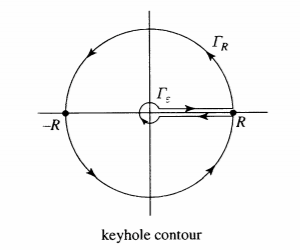
\includegraphics[width = 5.5cm]{Keyhole.PNG}
    \label{fig:key}
\end{wrapfigure}

For $\varepsilon > 0$ small and $R > 0$ large, we consider the keyhole domain $D$ consisting of $z$ in the slit plane $\C\backslash[0,\infty)$ satisfying $\varepsilon < |z| < R$. The function $f(z)$ has one pole in $D$, a double pole at $z = -1$. Using our residue rules we hav \begin{equation*}
    Res[z^a/(1+z)^2,-1] = \lim\limits_{z\rightarrow -1}a\frac{z^a}{z} = -ae^{\pi ia}
\end{equation*}
The residue theorem yields \begin{equation*}
    \int_{\partial D}f(z)dz = -2\pi iae^{\pi ia}
\end{equation*}
The integral around $\partial D$ breaks into the sum of four integrals, from $\varepsilon$ to $R$ along the top edge of the slit, around $\Gamma_R$, from $R$ back to $\varepsilon$ along the bottom edge of the slit, and around $\Gamma_{\varepsilon}$: \begin{equation*}
    \int_{\varepsilon}^R\frac{x^a}{(1+x)^2}dx + \int_{\Gamma_R}f(z)dz+\int_R^{\varepsilon}\frac{e^{2\pi ia}x^a}{(1+x)^2}dx+\int_{\Gamma_{\varepsilon}}f(z)dz
\end{equation*}
For the integrals over $\Gamma_R$ and $\Gamma_{\varepsilon}$, the ML-estimate gives \begin{align*}
    \left|\int_{\Gamma_R}\frac{z^a}{(1+z)^2}dz\right| &\leq \frac{R^a}{(R-1)^2}2\pi R\sim R^{a-1} \\
    \left|\int_{\Gamma_{\varepsilon}}\frac{z^a}{(1+z)^2}dz\right| &\leq \frac{\varepsilon^a}{(1-\varepsilon)^2}2\pi \varepsilon\sim \varepsilon^{a+1} \\
\end{align*}
Since $-1 < a < 1$, both these integrals tend to $0$ as $R\rightarrow \infty$ and $\varepsilon \rightarrow 0$. If we reverse the direction of the integral from $R$ to $\varepsilon$ and use our previous result we have \begin{equation*}
    -2\pi iae^{\pi ia} = (1-e^{2\pi ia})\int_{0}^{\infty}\frac{x^a}{(1+x)^2}dx
\end{equation*}
This yields the identity \begin{equation*}
    \int_0^{\infty}\frac{x^a}{(1+x)^2}dx = \frac{-2\pi iae^{\pi ia}}{1-e^{2\pi ia}} = \frac{2\pi ia}{e^{\pi ia}-e^{-\pi ia}} = \frac{\pi a}{\sin(\pi a)}
\end{equation*}


\begin{example}
    We wish to show that $$\int_0^{\infty}\frac{dx}{\sqrt{x}(x^2+1)} = \frac{\pi}{\sqrt{2}}$$
    Let $f(z) = \frac{z^{-1/2}}{z^2+1}$ where the root function is taken with the branch cut $[0,\infty)$. We use the keyhole contour depicted in the previous derivation. Notice $z = \pm i$ are the simple poles of $f(z)$ on the keyhole. We consider $z^{-1/2} = |z|^{-1/2}e^{-i\theta/2}$, where $\theta = \text{Arg}(z)$, so $0 < \theta < 2\pi$. Then $z^{-1/2} = \frac{1}{\sqrt{|z|}e^{i\theta/2}}$. Then, for the path along $\varepsilon$ to $R$ on the upper line $z^{-1/2} = 1/\sqrt{x}$, while on the lower line $z^{-1/2} = e^{2\pi i(-1/2)}/\sqrt{x} = -1/\sqrt{x}$. Next, we note that \begin{align*}
        \left|\int_{\Gamma_R}\frac{z^{-1/2}}{(1+z^2)}dz\right| &\leq \frac{\sqrt{R}}{(R^2-1)}2\pi R\sim R^{-1/2} \\
        \left|\int_{\Gamma_{\varepsilon}}\frac{z^{-1/2}}{(1+z^2)}dz\right| &\leq \frac{\varepsilon^{-1/2}}{(1-\varepsilon^2)}2\pi \varepsilon\sim \varepsilon^{1/2} \\
    \end{align*}
    Then as $R$ goes to infinity and $\varepsilon$ goes to $0$ both terms on the right go to $0$ so the integrals go to $0$. Now, we have the residues \begin{equation*}
        Res[1/(\sqrt{z}(z^2+1)),i] = \frac{1/(\sqrt{i}(i+i))}{1} = \frac{1}{2ie^{i\pi/4}}
    \end{equation*}
    and \begin{equation*}
        Res[1/(\sqrt{z}(z^2+1)),-i] = \frac{1/(\sqrt{-i}(-i-i))}{1} = \frac{e^{-3i\pi/4}}{-2i} 
    \end{equation*}
    Then, taking the limit we have that \begin{equation*}
        \int_{0}^{\infty}\frac{1}{\sqrt{x}(x^2+1)}dx - \int_0^{\infty}\frac{-1}{\sqrt{x}(x^2+1)}dx = 2\pi i\left(\frac{1}{2ie^{i\pi/4}}+\frac{e^{-3i\pi/4}}{-2i}\right) = \pi \left(e^{-i\pi/4}+e^{i\pi/4}\right)
    \end{equation*}
    Then simplifying we have \begin{equation*}
        \int_0^{\infty}\frac{dx}{\sqrt{x}(x^2+1)} = \pi\cos(\pi/4) = \frac{\pi}{\sqrt{2}}
    \end{equation*}
\end{example}
 

%%%%%%%%%%%%%%%%%%%% Section 1.7.5
\section{Fractional Residues}

Suppose $z_0$ is an isolated singularity of $f(z)$. For $\varepsilon > 0$ small, we consider the integral \begin{equation*}
    \int_{C_{\varepsilon}}f(z)dz
\end{equation*}
where $C_{\varepsilon}$ is the arc of the circle $|z-z_0| = \varepsilon$ subtended by a sector of aperture $\alpha$. if $\alpha = 2\pi$, then $C_{\varepsilon}$ is the full circle, and the integral is equal to $2\pi iRes[f(z),z_0]$. If the singularity of $f(z)$ is a simple pole, then we can calculate the limit of the integrals as $\varepsilon \rightarrow 0$ (as the arc encloses in on the singularity)

\begin{theorem}[Fractional Residue Theorem]
    If $z_0$ is a simple pole of $f(z)$, and $C_{\varepsilon}$ is an arc of the circle $|z-z_0| = \varepsilon$ of angle $\alpha$, then \begin{equation*}
        \lim\limits_{\varepsilon 0}\int_{C_{\varepsilon}}f(z)dz = \alpha iRes[f(z),z_0]
    \end{equation*}
\end{theorem}
\begin{proof}
    Since $f$ has a simple pole we have \begin{equation*}
        f(z) = \frac{A}{z-z_0}+g(z)
    \end{equation*}
    where $A = Res[f(z),z_0]$ and $g(z)$ is analytic at $z_0$. Then the arc $|z-z_0| = \varepsilon$ of angle $\alpha$ is parametrized by $z = z_0+\varepsilon e^{i\theta}$, $\theta_0\leq \theta\leq \theta_0+\alpha$. As the arc is a bounded subset and $g$ is analytic on the arc, it follows there exists $M > 0$ such that $|g(z)| < M$ for $|z-z_0| < \varepsilon$. Furthermore, the integral of the singular part is calculated \begin{equation*}
        \int_{C_{\varepsilon}}\frac{Adz}{z-z_0} = \int_{\theta_0}^{\theta_0+\alpha}\frac{Ai\varepsilon e^{i\theta}}{\varepsilon e^{i\theta}}d\theta = Ai\alpha
    \end{equation*}
    Note that \begin{equation*}
        \left|\int_{C_{\varepsilon}}g(z)dz\right| \leq M2\pi\varepsilon\rightarrow 0
    \end{equation*}
    by the ML-theorem, so the result follows.
\end{proof}


\begin{example}
    Let $\gamma = C_R\cup[-R,-1-\varepsilon]\cup C_{\varepsilon}\cup[-1+\varepsilon,R]$. This is a half-circular path with an idnentation around $z_0 = -1$. Here we assume $C_{\varepsilon}$ is a half-circle of radius $\varepsilon$ above the real axis. The aperature is $\pi$ (but clockwise), hence the fractional residue theorem yields \begin{equation*}
        \lim\limits_{\varepsilon\rightarrow 0}\int_{C_{\varepsilon}}\frac{dz}{(z+1)(z-i)} = -\pi iRes(1/[(z+1)(z-i)],-1) = -\pi i\frac{1}{-1-i} = \frac{\pi (i+1)}{2}
    \end{equation*}
    Now, observe that for $|z| = R > 1$, $$\left|\frac{1}{(z+1)(z-i)}\right| \leq \left|\frac{1}{||z|-|1||\cdot||z|-|i||}\right| = \frac{1}{(R-1)^2}$$
    Thus, by the ML-theorem \begin{equation*}
        \left|\int_{C_R}\frac{1}{(z+1)(z-i)}dz\right| \leq \frac{1}{(R-1)^2}\pi R \sim R^{-1}
    \end{equation*}
    which goes to $0$ as $R\rightarrow \infty$. Next, by Cauchy's Residue Theorem we have \begin{equation*}
        \int_{\gamma}\frac{1}{(z+1)(z-i)}dz = 2\pi iRes[1/[(z+1)(z-i)],i] = 2\pi i\frac{1}{i+1} = \pi(1+i)
    \end{equation*}
    Hence, as the limit $R\rightarrow \infty$ and $\varepsilon \rightarrow 0$, we find \begin{equation*}
        P.V.\int_{-\infty}^{\infty}\frac{dx}{(x+1)(x-i)} + \frac{\pi (i+1)}{2} = \pi(1+i)
    \end{equation*}
    so \begin{equation*}
        P.V.\int_{-\infty}^{\infty}\frac{dx}{(x+1)(x-i)} = \frac{\pi(i+1)}{2}
    \end{equation*}
\end{example}



%%%%%%%%%%%%%%%%%%%% Section 1.7.6
\section{Principal Values}

\begin{definition}
    An integral $\int_a^bf(x)dx$ is \Emph{absolutely convergent} if the (proper or improper) integral $\int_a^b|f(x)|dx$ is finite. The integral is \Emph{absolutely divergent} if $\int_a^b|f(x)|dx = \infty$.
\end{definition}

If an integral is absolutely divergent, there may not be an obvious way to assign a value to it (think of the relationship between absolutely and conditionally convergent series)

\begin{definition}
    Suppose $f(x)$ is continuous for $a \leq x < x_0$ and for $x_0 < x\leq b$. We define the \Emph{principal value} of the integral $\int_a^bf(x)dx$ to be \begin{equation*}
        PV\int_a^bf(x)dx = \lim\limits_{\varepsilon\rightarrow 0}\left(\int_a^{x_0-\varepsilon}+\int_{x_0+\varepsilon}^b\right)f(x)dx
    \end{equation*}
    provided that the limit exists.
\end{definition}
The principal value of the integral coincides with the usual value of the integral if $f(x)$ is absolutely integrable.



%%%%%%%%%%%%%%%%%%%% Section 1.7.7
\section{Jordan's Lemma}

\begin{lemma}[Jordan's Lemma]
    If $C_R$ is the semi-circular contour $z(\theta) = Re^{i\theta}$ for $0 \leq \theta \leq \pi$, in the upper half-plane, then \begin{equation*}
        \int_{C_R}|e^{iz}||dz| < \pi
    \end{equation*}
\end{lemma}
\begin{proof}
    Note $|e^{iz}| = e^{R\sin\theta}$ and $|dz| = Rd\theta$, so now we wish to show \begin{equation*}
        \int_{C_R}e^{R\sin\theta}d\theta < \frac{\pi}{R}
    \end{equation*}
    First, note that $\sin\theta$ is concave down on $0\leq \theta\leq \pi/2$, so the graph of $\sin\theta$ lies above the straight line connecting its endpoints, $\sin\theta >2\theta/\pi$, $0\leq\theta\leq \pi/2$. Thus \begin{align*}
        \int_0^{\pi}e^{-R\sin\theta}d\theta &= 2\int_0^{\pi/2}e^{-R\sin\theta}d\theta \leq 2 \int_0^{\pi/2}e^{-2R\theta/\pi}d\theta \\
        &= \frac{\pi}{R}\int_0^{1/R}e^{-t}dt < \frac{\pi}{R}\int_0^{\infty}e^{-t}dt = \frac{\pi}{R}
    \end{align*}
\end{proof}


\begin{example}
    Consider $\int_0^{\infty}\frac{\sin x}{x}dx$, and we calculate it using $f(z) = \frac{e^{iz}}{z}$ along an indented semi-circular path centered at $z = 0$ in the upper half plane. Notice for $|z| = R$, we have \begin{equation*}
        \left|\int_{C_R}\frac{e^{iz}}{z}dz\right| \leq \int_{C_R}\left|\frac{e^{iz}}{z}\right||dz| = \frac{1}{R}\int_{C_R}\left|e^{iz}\right||dz| < \frac{\pi}{R}
    \end{equation*}
    by Jordan's Lemma. Then as $R$ goes to $\infty$ this integral goes to $0$. Suppose $R$ goes to $\infty$ and $\varepsilon \rightarrow 0$, then Cauchy's residue and fractional residue then combine to yield \begin{equation*}
        \lim\limits_{\varepsilon\rightarrow 0}\int_{-R}^R\frac{e^{ix}}{x}dx - \pi iRes[e^{ix}/x, 0] + \lim\limits_{R\rightarrow \infty}\int_{C_R}\frac{e^{iz}}{z}dz = 0
    \end{equation*}
    hence, noting that the residue is $1$, we have \begin{equation*}
        \lim\limits_{R\rightarrow \infty}\left(\int_{-R}^{R}\frac{\cos x}{x}dx + i\int_{-R}^{R}\frac{\sin x}{x}dx\right) = \pi i
    \end{equation*}
    Note $\cos x/x$ is an odd function, hence the principal value of the integral vanishes. Thus, \begin{equation*}
        P.V.\int_{-\infty}^{\infty}\frac{\sin x}{x}dx = \pi\;\;\implies \int_0^{\infty}\frac{\sin x}{x}dx = \frac{\pi}{2}
    \end{equation*}
    since $\sin(x)/x$ is even.
\end{example}






